\documentclass[tikz]{standalone}


\usepackage{graphicx}
\usepackage{pxfonts}
\usetikzlibrary{arrows.meta}
\newcommand{\figf}{\bfseries\sffamily}
\definecolor{mycyan}{RGB}{0,255,255}

\begin{document}

\sffamily



\begin{tikzpicture}[anchor = north west]

	\clip (0,0) rectangle +(18,-13.5);

	\begin{scope}
		
		\node at (0.3,-0.1) {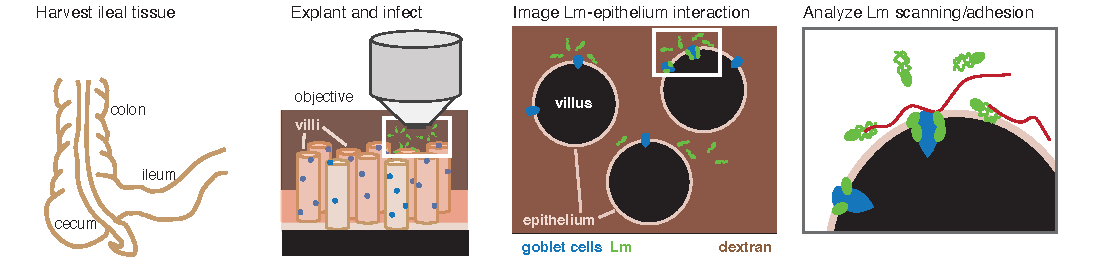
\includegraphics[width=17cm]{../img/schematic.pdf}};
		\node at (0,0) {\figf A};
	\end{scope}

	\begin{scope}[yshift=-4.5cm]
	\begin{scope}
		\clip (0,0) rectangle (+12.4,-11);
		\node at (-0.1,0) {\includegraphics[page=1,width=12.5cm]{../img/fig2_microscopy.pdf}};
		\begin{scope}[xshift=10.32cm, yshift=-3.45cm]
			\draw[fill=black] (0,0) rectangle +(2.1,-1.05);
			\draw [-{latex[scale=1]},line width=1.2pt,mycyan](0.15,-.2) -- +(0.2,0);
			\node[mycyan,anchor=west] at (0.3,-.2){\tiny Lm-37 tracks};
			\draw [-{latex[scale=2]},line width=1.2pt,white](0.15,-.5) -- +(0.2,0);
			\node[white,anchor=west] at (0.3,-.5){\tiny GC};
			\draw [-{latex[scale=2]},line width=1.2pt,yellow](0.15,-.8) -- +(0.2,0);
			\node[yellow,anchor=west] at (0.3,-.8){\tiny Lm-37};
		\end{scope}
		\begin{scope}[xshift=10.32cm, yshift=-7.82cm]
			\draw[fill=black] (0,0) rectangle +(2.1,-1.05);
			\draw [-{latex[scale=2]},line width=1.2pt,white](0.15,-.5) -- +(0.2,0);
			\node[white,anchor=west] at (0.3,-.5){\tiny GC};
			\draw [-{latex[scale=2]},line width=1.2pt,yellow](0.15,-.8) -- +(0.2,0);
			\node[yellow,anchor=west] at (0.3,-.8){\tiny Lm-RT};
		\end{scope}
		%\node at (0,0) {\figf A};
	\end{scope}
		
	\begin{scope}[xshift = 12.5cm]
		\node at (0,0.18) {\includegraphics{../plots/panelsHI.pdf}};
		\node at (0,-0.1) {\figf H};
		\node at (0,-4.5) {\figf I};
	\end{scope}
	\end{scope}
	

\end{tikzpicture}

\end{document}